\section{Orbifold bases before and after contraction}\label{sec:composition}

We locate the error in \cite[Claim 7.17]{CDHP2026} by instantiating its
models on the surface just constructed. This also explains why neither
an isogeny of the elliptic base nor a further allowed source modification
repairs the fibre-specialness statement.

For a composition of fibrations in the preceding orbifold setting,
\[
 (Y,D)\xrightarrow{c}\bar X\xrightarrow{\bar j}J,
\]
one must distinguish the two divisors
\begin{equation}\label{eq:two-bases}
 \Delta(\bar j\circ c,D)
 \quad\hbox{and}\quad
 \Delta\bigl(\bar j,\Delta(c,D)\bigr).
\end{equation}
An exceptional divisor for $c$ is omitted when constructing
$\Delta(c,D)$. If it dominates a divisor of $J$, however, it participates
in the direct infimum for $\bar j\circ c$. Thus equality in
\eqref{eq:two-bases} needs a hypothesis controlling precisely those
divisors. This issue is already present in Campana's composition rule:
the direct base divisor is at most the iterated one, and equality holds
when $c:(Y,D)\to(\bar X,\Delta(c,D))$ is an orbifold morphism
\cite[arXiv version, Proposition 3.13]{Campana2011}. The retained
exceptional divisors in our example make the inequality strict.

In our example, take $c=b:Y\to S$, $J=\PP^1$ and
$\bar j=\operatorname{pr}_{\PP^1}:S\to\PP^1$. The only divisor of $Y$
dominating $H_i\subset S$ is $D_i$, with multiplicity one and boundary
multiplicity infinity. Therefore
\begin{equation}\label{eq:iterated-base}
 \Delta(b,D)=\sum_iH_i,
 \qquad
 \Delta\Bigl(\bar j,\sum_iH_i\Bigr)=\sum_iq_i.
\end{equation}
By contrast, \eqref{eq:j-base-zero} gives
\begin{equation}\label{eq:direct-base}
 \Delta(\bar j\circ b,D)=0.
\end{equation}
The two answers differ at every $q_i$: the direct multiplicity is
$\min(\infty,1)=1$, whereas the iterated multiplicity is $\infty$. Figure~\ref{fig:retained-exceptional} records
which component is lost at the intermediate step.

\begin{figure}[tbp]
\centering
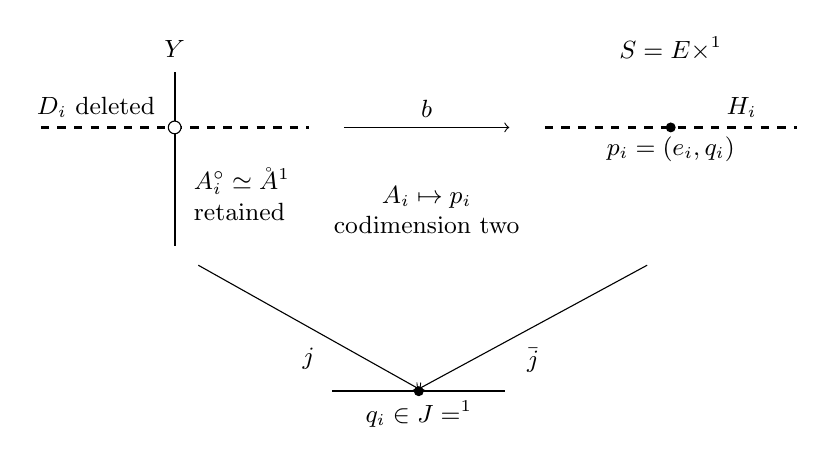
\begin{tikzpicture}[x=1cm,y=1cm,font=\small]
  \node at (0,2) {$Y$};
  \draw[dashed,thick] (-1.7,1)--(1.7,1);
  \node[above] at (-1,1) {$D_i$ deleted};
  \draw[thick] (0,-.5)--(0,1.7);
  \filldraw[fill=white] (0,1) circle (2.3pt);
  \node[right,align=left] at (.12,.15)
    {$A_i^\circ\simeq\AA^1$\\retained};
  \draw[->] (2.15,1)--(4.25,1) node[midway,above] {$b$};
  \node[align=center] at (3.2,-.05)
    {$A_i\mapsto p_i$\\codimension two};
  \node at (6.3,2) {$S=E\times\PP^1$};
  \draw[dashed,thick] (4.7,1)--(7.9,1);
  \fill (6.3,1) circle (1.8pt);
  \node[above] at (7.2,1) {$H_i$};
  \node[below] at (6.3,1) {$p_i=(e_i,q_i)$};
  \draw[->] (.3,-.75)--(3.1,-2.32)
    node[midway,below=4pt] {$j$};
  \draw[->] (6,-.75)--(3.1,-2.32)
    node[midway,below=4pt] {$\bar j$};
  \draw[thick] (2,-2.35)--(4.2,-2.35);
  \fill (3.1,-2.35) circle (1.8pt);
  \node[below] at (3.1,-2.35) {$q_i\in J=\PP^1$};
\end{tikzpicture}
\smallskip
\[
\begin{array}{c|c|c}
 & \text{multiplicity at }q_i & \text{boundary coefficient}\\ \hline
\text{direct base} & \min\{\infty,1\}=1 & 0\\
\text{iterated base} & \infty & 1
\end{array}
\]
\caption{Incidence schematic showing the two routes to the same point
$q_i$. The horizontal arrow is
the blowdown of complete surfaces: the retained $A_i^\circ$ maps to a
point on $H_i$. The hollow point $A_i\cap D_i$ is removed from $X$.
The divisor $A_i$ is omitted from the intermediate orbifold base because
$b(A_i)$ has codimension two in $S$, but contributes multiplicity one
to the direct base over $q_i$.}
\label{fig:retained-exceptional}
\end{figure}


\subsection{The models occurring before Claim 7.17}
We next check that this discrepancy occurs on the models used in the
cited claim. The \emph{relative core} used there has special general
fibres, and its base pair has general-type general fibres over $E$.
In our case it can be represented
by the identity of $Y$: the identity has point fibres, while the general
fibres of $(Y,D)\to E$ are the log-general-type punctured projective
lines. The identity is a neat and high model in the
terminology of \cite[Definitions 2.3 and Theorem 2.10]{CDHP2026}.
The log-canonical calculation \eqref{eq:log-canonical} gives the
Kodaira dimension one required in the subsequent reduction. General
Iitaka fibres are complete elliptic curves mapping isomorphically to
$E$.

An isogeny $E'\to E$ pulls the construction back to the blowup of
$E'\times\PP^1$ at all preimages of the centres. It is finite \'etale on
the entire pair. The boundary is the pullback of $D$, the exceptional
curves still have coefficient zero, and the log-canonical divisor is
still pulled back from $\OO_{\PP^1}(n-2)$. Thus the minimizing-isogeny
step in \cite[Equation (7.15.2)]{CDHP2026} leaves the relative-core
canonical dimension equal to one and retains the exceptional divisors.

For the birational contraction in \cite[Proposition 7.6]{CDHP2026},
we can take $b:Y\to S$. Indeed, the fixed semiabelian subvariety in
that construction is the image in $E$ of a general Iitaka fibre, hence
$E$ itself. The quotient is a point, and the resulting contracted
family is $\PP^1\times E\simeq S$. This product is smooth over all of $J$,
so the open set $J^0$ used for the smooth contracted family can be
taken to be $J$; its complement $\partial J$ is empty.
On the contracted
space $S$, the boundary $\sum_iH_i$ has the general-type orbifold base
shown in \eqref{eq:iterated-base}. This is consistent with
\cite[Claim 7.7]{CDHP2026}; the difficulty is transferring that
conclusion back to $(Y,D)$.

The proof next makes a birational change $J'\to J$ so that the main
component of $Y\times_JJ'$ is flat \emph{over $J'$}. Here
$j:Y\to\PP^1$ is already flat. One way to see this is that at each
point of the smooth curve base its local ring is a discrete valuation
ring, and the local rings of the dominant smooth integral source are
torsion-free modules over it. Torsion-free modules over a discrete
valuation ring are flat. A smooth birational model of the complete
curve $J=\PP^1$ is isomorphic to $J$. The choices in the proof can
therefore be instantiated with
\[
 J'=J,\qquad\bar X'=\bar X\times_JJ'=S,\qquad
 \widetilde X=S,\qquad\widetilde Y=Y.
\]
Here $\nu:\widetilde Y\to Y$ is the source modification and
$\mu:\widetilde X\to\bar X'$ is the resolution of the intermediate
target. Both are identities, and the maps to that target and to $J'$
are
\[
 \nu=\operatorname{id}_Y,\quad\mu=\operatorname{id}_S,\quad
 \widetilde c=b,\quad\widetilde j=\bar j.
\]
The boundary in \cite[Equation (7.16.7)]{CDHP2026} is then exactly $D$,
because there are no $\nu$-exceptional divisors to add.

\subsection{The change of flatness target}
Claim 7.17 asserts equality of the two divisors in
\eqref{eq:two-bases} on the resulting models. Its proof treats every
$\widetilde c$-exceptional divisor as having infinite boundary
multiplicity. To justify this, it uses flatness of
\[
 (Y\times_JJ')_{\mathrm{main}}\longrightarrow\bar X'
\]
although the preceding construction arranged flatness over $J'$.
These are different morphisms. In the displayed instance the former
map is the blowdown $b:Y\to S$. Its fibres are points away from the
centres and curves over the centres, so it is not flat. The divisors
$A_i$ are exceptional for $\widetilde c=b$ but are not exceptional for
$\nu=\operatorname{id}_Y$; they have boundary multiplicity $1$, not
$\infty$. Omitting them from the direct infimum is precisely what turns
\eqref{eq:direct-base} into the incorrect answer
\eqref{eq:iterated-base}.

This is a numerical failure of the asserted equality, as well as a
failure of the stated justification. Adding the $A_i$ to the boundary
would turn the blowdown into an orbifold morphism, but it would replace
$X$ by
\[
 E\times(\PP^1\setminus Q),
\]
which is not special and has group $\Z^2\times F_{n-1}$, where
$F_{n-1}$ is the free group of rank $n-1$.
Alternatively, making the intermediate target remember the blowups
retains the reducible fibres $D_i+A_i$ and restores the zero orbifold
base; the general-type base computed on the contracted model is then
lost. Neither modification establishes the original assertion for
the original open variety.

The counterexample and this calculation concern the fixed version
\cite{CDHP2026}. Its Theorem A is a separate assertion about linear
representation images. Our proof of that conclusion in
Section~\ref{sec:linear} uses independent inputs and does not use the
fibre-specialness assertion.
